\documentclass[11pt]{article}
\usepackage{graphicx}
\usepackage[utf8]{inputenc}
\usepackage{enumerate}
\usepackage{multirow,tabularx}
\usepackage{caption}
\usepackage{subfigure}
\usepackage[T1]{fontenc}
\usepackage{mathptmx}
\usepackage[a4paper, left=2cm, right=2cm, top=2.5cm, bottom=2.5cm, headsep=1.2cm]{geometry} 
\usepackage[rightcaption]{sidecap}
\usepackage{float}
\usepackage{url}

\begin{document}

\begin{titlepage}

	\begin{center}
    
\includegraphics[width=7cm]{Logo-PW-duze.jpg} \\
    [10mm]
	\line(1,0){435} \\
	[8mm]
	\huge{\textsc{Metody Komputerowe w Spalaniu}} \\
	\line(1,0){435} \\
	[15mm]
    \LARGE{\textbf{Autoignition of methane - air mixture for different initial temperature, pressure and equivalence ratio}} \\
	[50mm]
	\Large{Mateusz Więcław}\\
    \Large{271360}\\
    [25mm]
    \large{Aerospace Engineering}\\
    [3mm]
    \large{Warsaw, 26.04.2017}\\
    \end{center}
    
\end{titlepage}

\newpage

\section{Abstract.}
The purpose of the project was to conduct a study of Chapman-Jouget detonation of a methane oxygen mixture for different initial temperature, pressure and equivalent ratio, using Cantera and SDToolbox software. The results of the study are several plots, showing influence of these parameters on C-J detonation speed, temperature, pressure and density.

\section{Mathematic model.}
There are several mechanisms that can be used for C-J detonation parameters. For the needs of the study, we used the one called 'Hai Wang Mechanism'. It uses conservation of energy rules:\\
\begin{enumerate}
\item \(\rho_1 w_1 = \rho_2 w_2\)
\item \(P_1 + \rho_1 (w_1)^2 = P_2 + \rho_2 (w_2)^2\)
\item \(h_1 +  {w_1^2}/2 = h_2 +  {w_2^2}/2\)
\end{enumerate}

The calculations were held for 10 different temperatures, pressures and $\phi (10x10x10)$. It took couple of minutes (~2-3) to calculate it. The more accurate we want the calculations to be, the more iterations we have to make and the more time it takes. For the purpose of this project, 10x10x10 is more than enough.

\section{Results and plots.}









\subsection{Results for $P=1013,25hPa$,  $\phi =1$ and different initial temperatures.}
 
 \begin{figure} [H]
	\begin{center}
    	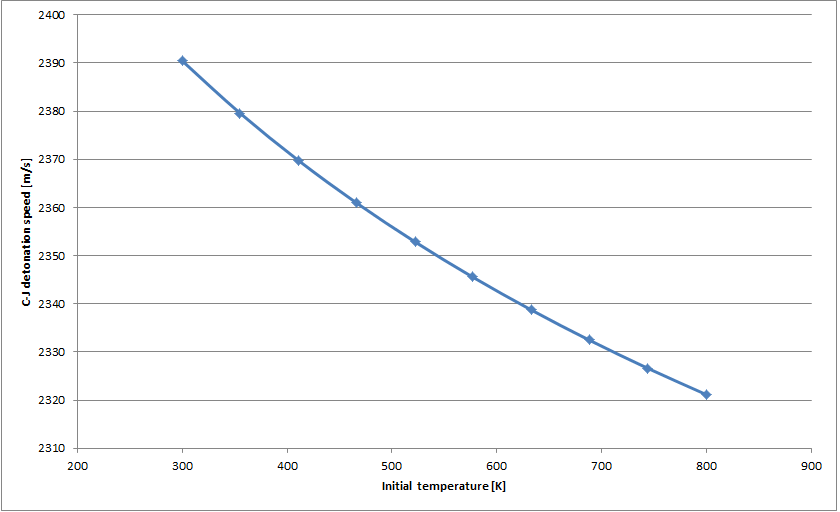
\includegraphics[width=0.8\textwidth]{ftemp_speed}
        \caption{Influence of initial temperature on  C-J detonation speed.}
    \end{center}
\normalsize
{We observe a severe drop of the C-J detonation speed with a rise of the temperature.}
\end{figure}


 \begin{figure} [H]
	\begin{center}
    	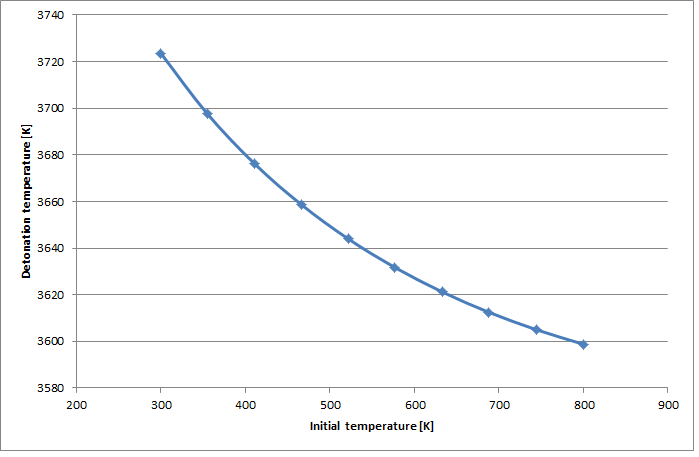
\includegraphics[width=0.8\textwidth]{ftemp_temp}
        \caption{Influence of initial temperature on detonation temperature.}
    \end{center}
\normalsize
{influence of initial temperature on final temperature. Starting with 300K, a decrease of a final temperature is noticed. For initial temperature of 300K detonation temperature is 3725K and for initial temperature of 800K detonation temperature is 3600K.}
\end{figure}

 \begin{figure} [H]
	\begin{center}
    	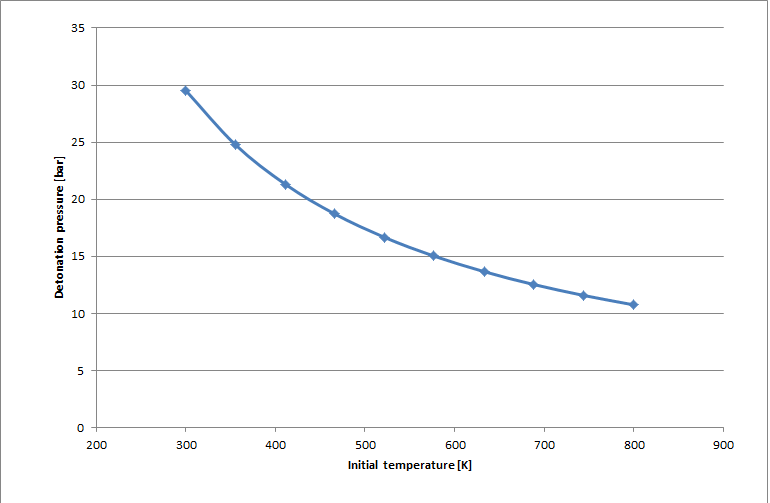
\includegraphics[width=0.8\textwidth]{ftemp_press}
        \caption{Influence of initial temperature on detonation pressure.}
    \end{center}
\normalsize
{influence of initial temperature on detonation pressure. Starting with 300K, a decrease of detonation pressure is noticed. }
\end{figure}

 \begin{figure} [H]
	\begin{center}
    	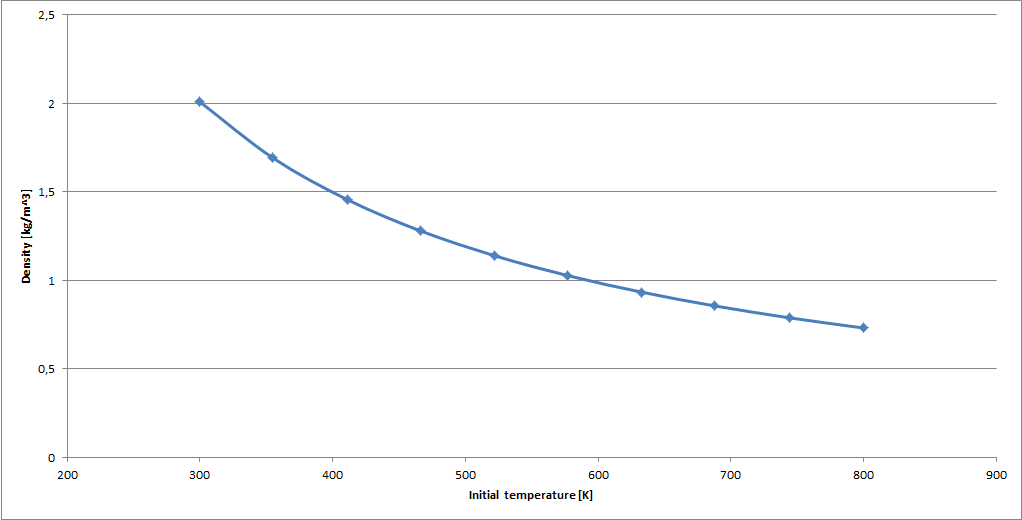
\includegraphics[width=0.8\textwidth]{ftemp_dens}
        \caption{Influence of initial temperature on detonation density.}
    \end{center}
\normalsize
{influence of initial temperature on detonation density. Starting with 300K, a decrease of detonation density is noticed. }
\end{figure}










\subsection{Results for $T=300K$, $\phi =1$ and different initial pressure.}


 \begin{figure} [H]
	\begin{center}
    	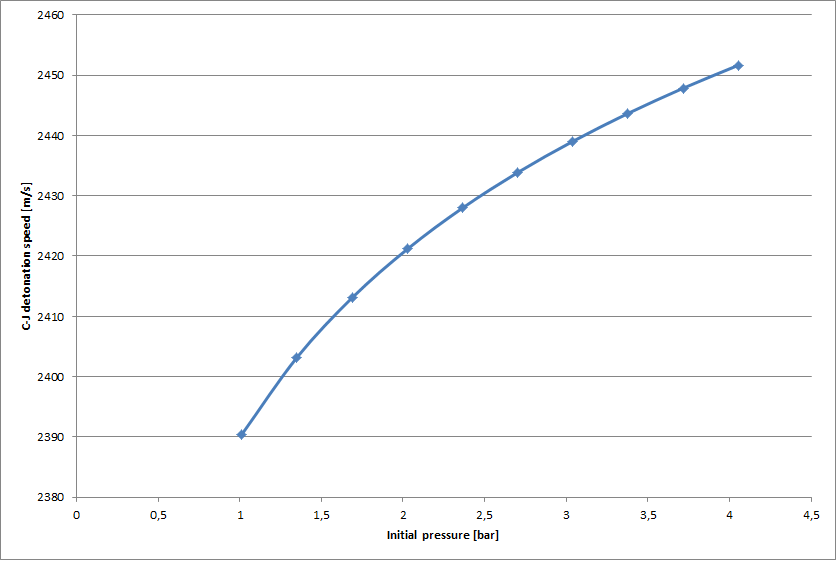
\includegraphics[width=0.8\textwidth]{fpress_speed}
        \caption{Influence of initial pressure on  C-J detonation speed.}
    \end{center}
\normalsize
{We observe an increase of the C-J detonation speed with a rise of the pressure.}
\end{figure}


 \begin{figure} [H]
	\begin{center}
    	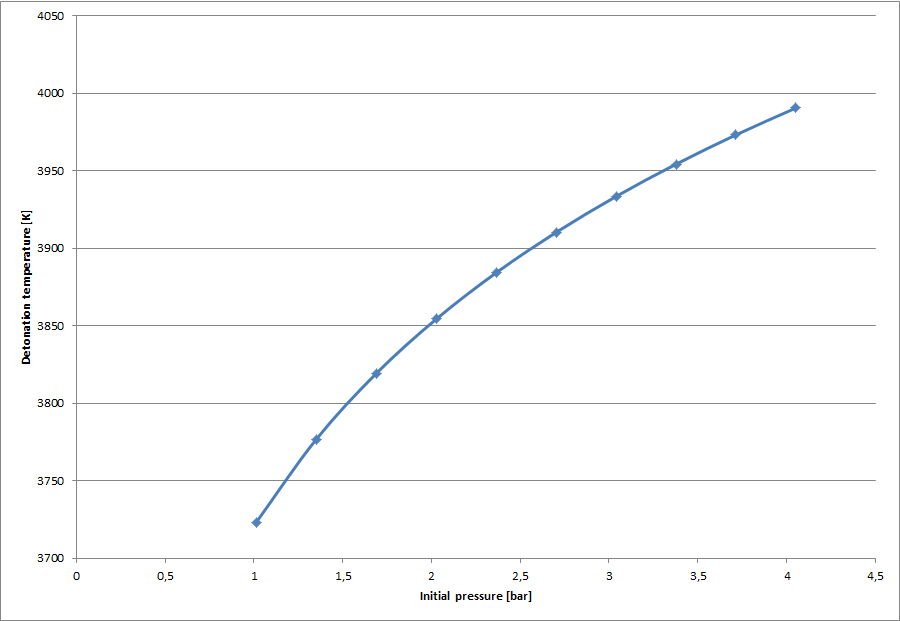
\includegraphics[width=0.8\textwidth]{fpress_temp}
        \caption{Influence of initial pressure on detonation temperature.}
    \end{center}
\normalsize
{Influence of initial temperature on final temperature. Starting with 300K, a decrease of a final temperature is noticed. For initial temperature of 300K detonation temperature is 3725K and for initial temperature of 800K detonation temperature is 3600K.}
\end{figure}

 \begin{figure} [H]
	\begin{center}
    	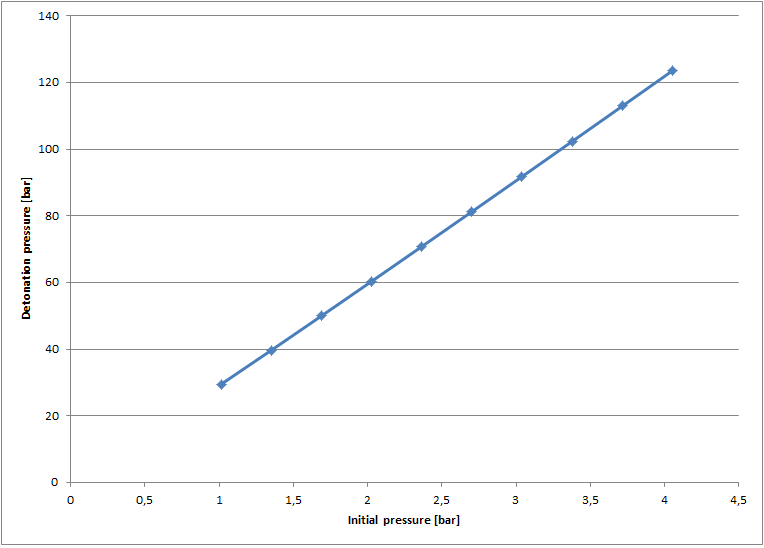
\includegraphics[width=0.8\textwidth]{fpress_press}
        \caption{Influence of initial pressure on detonation pressure.}
    \end{center}
\normalsize
{influence of initial temperature on detonation pressure. Starting with 300K, an increase of detonation pressure is noticed. }
\end{figure}

 \begin{figure} [H]
	\begin{center}
    	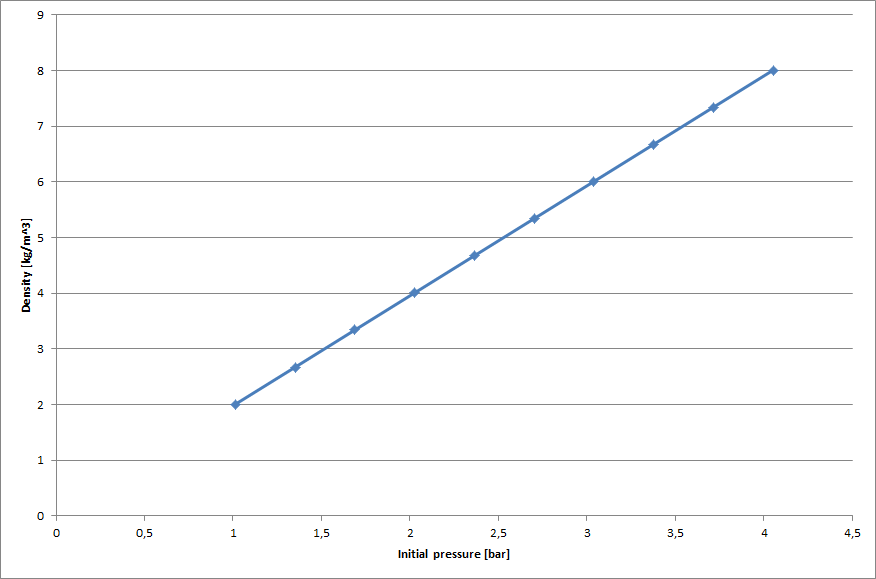
\includegraphics[width=0.8\textwidth]{fpress_dens}
        \caption{Influence of initial temperature on detonation density.}
    \end{center}
\normalsize
{influence of initial temperature on detonation density. Starting with 300K, a decrease of detonation density is noticed. }
\end{figure}











\subsection{Results for $T=300K$, $P=1013,25hPa$ and different equivalent ratio values ($\phi$).}

 
 \begin{figure} [H]
	\begin{center}
    	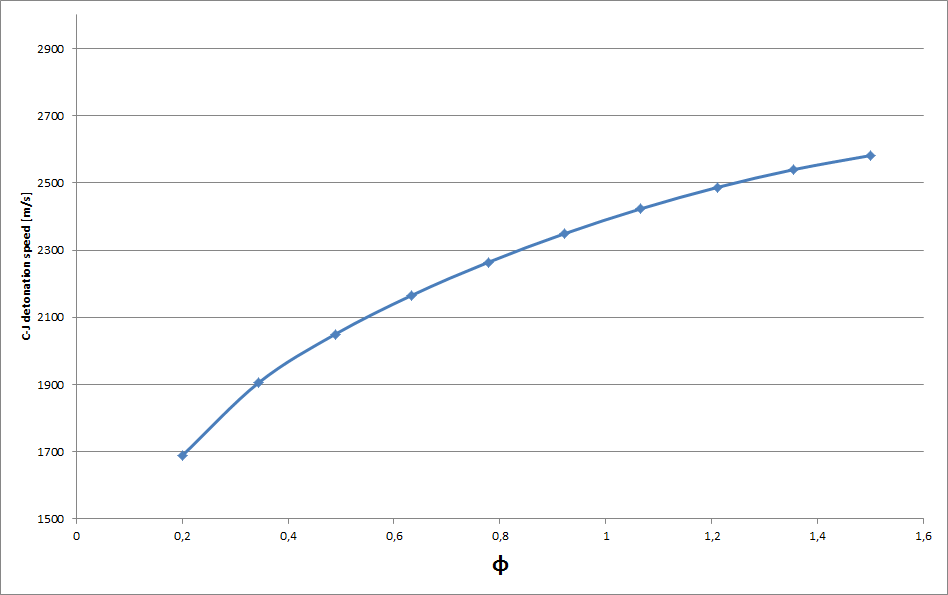
\includegraphics[width=0.8\textwidth]{ffi_speed}
        \caption{Influence of equivalent ratio on  C-J detonation speed.}
    \end{center}
\normalsize
{We observe an increase of the C-J detonation speed with a rise of equivalent ratio.}
\end{figure}


 \begin{figure} [H]
	\begin{center}
    	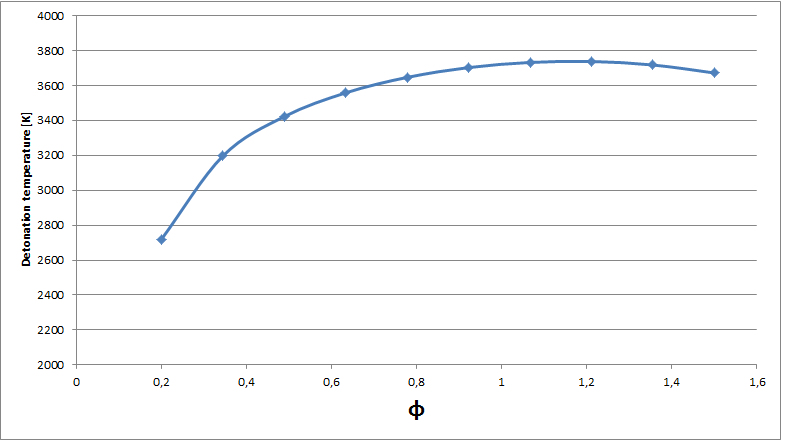
\includegraphics[width=0.8\textwidth]{ffi_temp}
        \caption{Influence of equivalent ratio on detonation temperature.}
    \end{center}
\normalsize
{influence of equivalent ratio on final temperature.}
\end{figure}

 \begin{figure} [H]
	\begin{center}
    	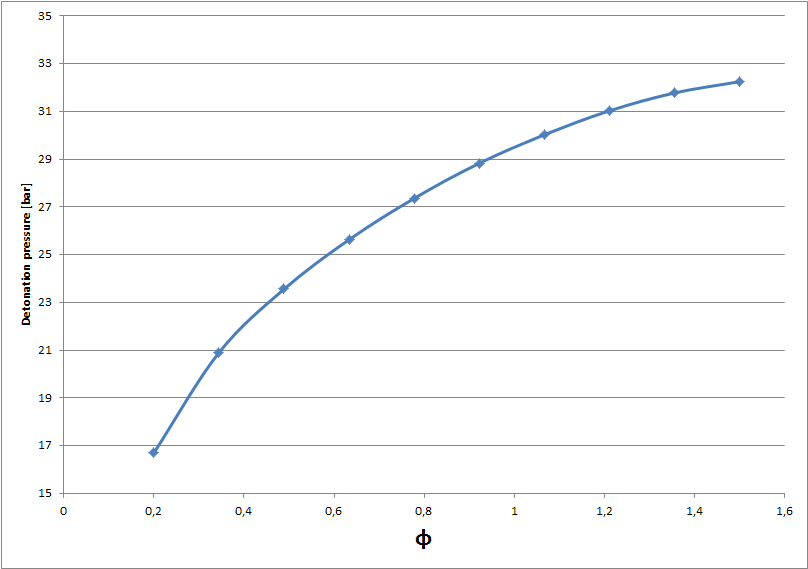
\includegraphics[width=0.8\textwidth]{ffi_press}
        \caption{Influence of equivalent ratio on detonation pressure.}
    \end{center}
\normalsize
{influence of equivalent ratio on detonation pressure.}
\end{figure}

 \begin{figure} [H]
	\begin{center}
    	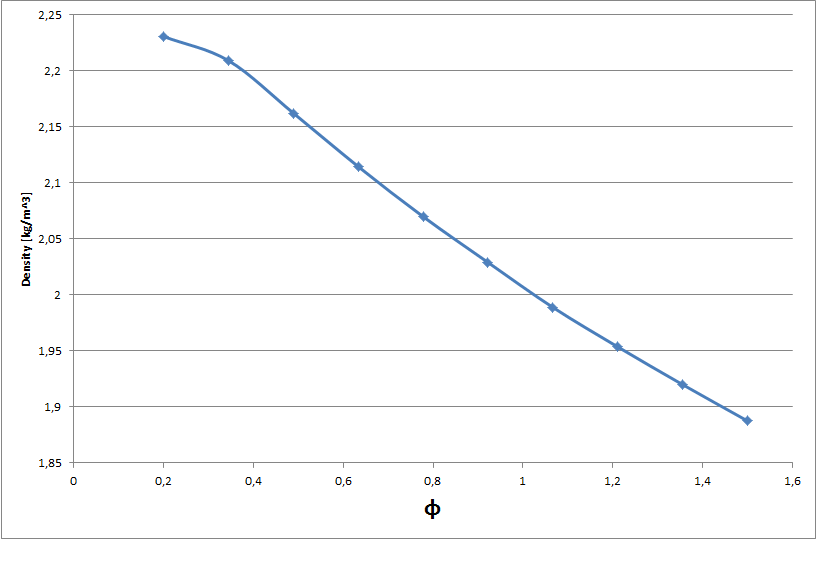
\includegraphics[width=0.8\textwidth]{ffi_density}
        \caption{Influence of equivalent ratio on detonation density.}
    \end{center}
\normalsize
{influence of initial temperature on detonation density. Starting with 300K, a decrease of detonation density is noticed. }
\end{figure}







\section{Overall.}
The study gives information about the behavior of detonation parameters as a function of temperature, pressure and $\phi$. The definition of autoignition proposed in the mathematical model is the most commonly used one. The data read from the plots are just approximations of the actual state. The more precise data can be read from the .csv file ($MW-Autoignition_Methane.csv$ attached to a report). This file contains information about the lowest temperature of autoignition.

\section{References.}
\begin{enumerate}
\item $CANTERA\_HandsOn.pdf$
\item Prediction of auto-ignition temperatures and delays for gas turbine applications. \\
\url{http://proceedings.asmedigitalcollection.asme.org/proceeding.aspx?articleid=2428119}
\end{enumerate}


\end{document}